\subsection{Testing y pruebas} \mbox{} \vspace{5pt}

Las pruebas que se realizaron para que efectivamente podamos determinar el correcto funcionamiento del Monitor, la gestión de la cola de cortesía y la resolución de conflictos mediante la aplicación de una Política fue con la ayuda de la Red de Petri sumamente conocida como Productor-Consumidor. Esta se tomó cómo referencia ya que permite evaluar los problemas de sincronización, concurrencia y gestión de los recursos, entonces, nos pareció un buen puntapié para validar el funcionamiento con un modelo conocido y sumamente usado.

\begin{figure}[H]
   \centering
   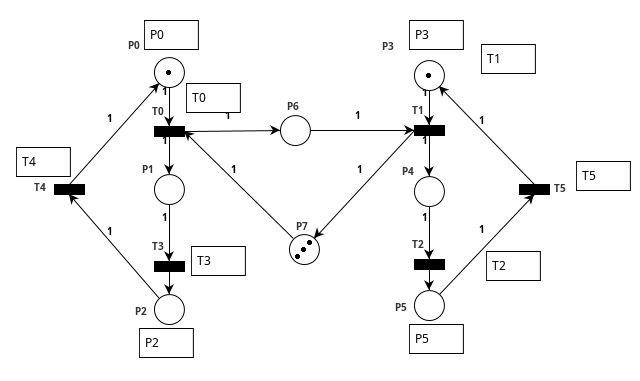
\includegraphics[width=0.9\linewidth]{images/rdp_prod_cons.png}
   \caption{Red de Petri productor-consumidor}
   \label{fig:rdp_prod_cons}
\end{figure}

Se plantearon los siguientes casos:

\begin{testtableformat}
   \hline \rowcolor{test_header_color}
       Test ID             & TC\_04\_00 \\
   \hline
       Tipo de test        & Test unitario \\
   \hline
       Objeto de prueba    & Disparar las transiciones sensibilizadas del Productor \\
   \hline
       Nombre              & Ejecución del productor \\
   \hline
       Descripción         & Realizar el disparo de las transiciones sensibilizadas del productor teniendo como máximo 3 (tres) tokens disponibles para producir\\
   \hline
       Precondición        & PRECOND\_D \\
   \hline
       Pasos del test      & \begin{enumerate}
                             \item Instanciar a la clase monitor con la red productor-consumidor
                             \item Obtener el vector de transiciones sensibilizadas 
                             \item Ejecutar un disparo de la transición sensibilizada 
                             \item Adquirir el marcado saliente y compararlo con un programa de análisis de redes de Petri 
                             \end{enumerate}\\
   \hline
       Resultado esperado  & El marcado en ambos casos debe coincidir \\
   \hline
       Resultado obtenido  & El marcado de la red obtenido por la clase monitor y el programa de análisis de redes de Petri son iguales, por lo tanto, se verifica su adecuado funcionamiento \\
   \hline
       Observaciones       & -\\
   \hline
\end{testtableformat}

\begin{testtableformat}
   \hline \rowcolor{test_header_color}
       Test ID             & TC\_04\_01 \\
   \hline
       Tipo de test        & Test unitario \\
   \hline
       Objeto de prueba    & Disparar las transiciones sensibilizadas del consumidor \\
   \hline
       Nombre              & Ejecución del consumidor \\
   \hline
       Descripción         & Realizar el disparo de las transiciones sensibilizadas del consumidor teniendo como máximo 3 (tres) recursos disponibles generados por el productor\\
   \hline
       Precondición        & PRECOND\_D \\
   \hline
       Pasos del test      & \begin{enumerate} 
                             \item Instanciar a la clase monitor con la red productor-consumidor 
                             \item Obtener el vector de transiciones sensibilizadas 
                             \item Ejecutar un disparo de la transición sensibilizada 
                             \item Adquirir el marcado saliente y compararlo con un programa de analisis de redes de petri 
                             \end{enumerate}\\
   \hline
       Resultado esperado  & El marcado en ambos casos debe coincidir \\
   \hline
       Resultado obtenido  & El marcado de la red obtenido por la clase monitor y el programa de análisis de redes de Petri son iguales, por lo tanto, se verifica su adecuado funcionamiento \\
   \hline
       Observaciones       & -\\
   \hline
\end{testtableformat}

\begin{testtableformat}
   \hline \rowcolor{test_header_color}
       Test ID             & TC\_04\_02 \\
   \hline
       Tipo de test        & Test unitario \\
   \hline
       Objeto de prueba    & Disparar una transición con política de decisión \\
   \hline
       Nombre              & Ejecución de una transición con política definida \\
   \hline
       Descripción         & En en el caso donde tanto el productor cómo el consumidor pueden disparar una transición, la idea es evaluar la política de la transición del consumidor para que tenga prevalencia sobre el productor ante una situación indeterminista \\
   \hline
       Precondición        & PRECOND\_E \\
   \hline
       Pasos del test      & \begin{enumerate} 
                             \item Instanciar a la clase monitor con la red productor-consumidor 
                             \item Generar una situación de equidad donde ambos recursos puedan disparar su transición 
                             \item Obtener el vector de transiciones sensibilizadas 
                             \item Evaluar la política de las transiciones sensibilizada y elegir cual disparar 
                             \item Ejecutar un disparo de la transición elegida 
                             \item Adquirir el marcado saliente y compararlo con un programa de análisis de redes de petri 
                             \end{enumerate}\\
   \hline
       Resultado esperado  & El marcado actual en ambos casos debe coincidir y la transición disparada debe ser la del consumidor \\
   \hline
       Resultado obtenido  & El marcado de la red obtenido por la clase monitor y el programa de análisis de redes de Petri son iguales, por lo tanto, se verifica su adecuado funcionamiento \\
   \hline
       Observaciones       & -\\
   \hline
\end{testtableformat}

\begin{testtableformat}
   \hline \rowcolor{test_header_color}
       Test ID             & TC\_04\_03 \\
   \hline
       Tipo de test        & Test integración \\
   \hline
       Objeto de prueba    & Realizar movimientos con el robot dentro del mapa, el robot sólo va a avanzar cuando la red de Petri haya hecho la solicitud de disparo y haya verificado que el robot no se encuentra bloqueado.\\
   \hline
       Nombre              & Desplazamientos del robot controlado por el Monitor\\
   \hline
       Descripción         & Para que el robot avance de una celda a otra y realice el desplazamiento definido (punto inicial y final) debe ser autorizado y coordinado por el monitor que controla la red de Petri.\\
   \hline
       Precondición        & PRECOND\_E \\
   \hline
       Pasos del test      & \begin{enumerate}
                             \item Indicar los puntos de inicio y final del robot
                             \item Esperar que el Monitor dispare la transición sensibilizada
                             \item El robot recibe la orden de avanzar a la celda libera
                             \item El robot envía una señal de llegada a la celda (plaza)
                             \item Se dispara la siguiente transición sensibilizada
                             \item Este proceso se repite hasta que el robot llegue a su destino
                             \end{enumerate}\\
   \hline
       Resultado esperado  & El robot pueda completar su desplazamiento definido por el usuario\\
   \hline
       Resultado obtenido  & La red de Petri al no bloquearse permite que todas las transiciones sensibilizadas se puedan disparar y por ende que el robot pueda desplazarse por todas las celdas (plazas) involucradas en su recorrido\\
   \hline
       Observaciones       & -\\
   \hline
\end{testtableformat}

\begin{testtableformat}
    \hline \rowcolor{test_header_color}
        Test ID             & TC\_04\_04 \\
    \hline
        Tipo de test        & Test de sistema \\
    \hline
        Objeto de prueba    & Comunicación inalámbrica - PID - Modelo cinemático - Odometría - Seguidor de línea magnética - Modelo del mapa - Calculador de trayectorias - Red de Petri - Monitor\\
    \hline
        Nombre              & Prueba de sistema integrado\\
    \hline
        Descripción         & Comprobar que el robot se puede desplazar por el mapa gestionado por el marcado de la red de Petri\\
    \hline
        Precondición        & PRECOND\_G \\
    \hline
        Pasos del test      & \begin{enumerate}
                              \item Indicar los puntos de inicio y final del robot en el mapa
                              \item Calcular la secuencia de disparos del Monitor
                              \item Esperar que el Monitor dispare la transición sensibilizada
                              \item El robot recibe la orden de avanzar a la celda (plaza) liberada
                              \item El robot envía una señal de llegada a la celda (plaza) destino
                              \item Se dispara la siguiente transición sensibilizada
                              \item Este proceso se repite hasta que el robot llegue a su destino
                              \end{enumerate}\\
    \hline
        Resultado esperado  & El robot pueda completar su desplazamiento definido por el usuario\\
    \hline
        Resultado obtenido  & La red de Petri al no bloquearse permite que todas las transiciones sensibilizadas se puedan disparar y por ende que el robot pueda desplazarse por todas las celdas (plazas) involucradas en su recorrido\\
    \hline
        Observaciones       & Se probó recorridos de 4 de metros por limitaciones de espacio\\
    \hline
 \end{testtableformat}